\chapter{Witt rings and $NK$-groups}
References:
\begin{itemize}
    \item[part 1] J.\,P.\ Serre, Local fields.
    \item[part 1] Daniel\ Finkel, An overview of Witt vectors.
    \item[part 2] Hendrik\ Lenstra, Construction of the ring of Witt vectors.
    \item[part 2] Barry\ Dayton, Witt vectors, the Grothendieck Burnside ring, and Necklaces.
	\item[part 3] C.\,A.\ Weibel, Mayer-Vietoris sequences and module structures on $NK_*$, pp. 466–493 in Lecture Notes in Math. 854, Springer-Verlag, 1981.
	\item[part 3] D.\, R.\ Grayson, Grothendieck rings and Witt vectors.
	\item[part 3] C.\,A.\ Weibel, The $K$-Book: An introduction to algebraic $K$-theory.
\end{itemize}
\begin{figure}[htbp]
	\centering
	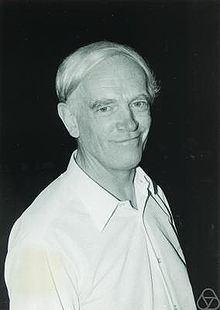
\includegraphics[width=0.3\textwidth]{./figures/Witt}
	\caption{Ernst Witt}
\end{figure}
\paragraph{Ernst Witt} % (fold)
\label{par:ernst_witt}
Ernst Witt\index{Ernst Witt} (June 26, 1911--July 3, 1991) was a German mathematician, one of the leading algebraists of his time. Witt completed his Ph.D. at the University of G\"{o}ttingen in 1934 with Emmy Noether. Witt's work has been highly influential. His invention of the Witt vectors clarifies and generalizes the structure of the $p$-adic numbers. It has become fundamental to $p$-adic Hodge theory. For more information, see \url{https://en.wikipedia.org/wiki/Ernst_Witt} and \url{http://www-history.mcs.st-andrews.ac.uk/Biographies/Witt.html}.
% paragraph ernst_witt (end)

%
%
%
\section{$p$-Witt vectors} % (fold)
\label{sec:p_witt_vectors}
In this section we introduce $p$-Witt vectors. Witt vectors generalize the $p$-adics and we will see all $p$-Witt vectors over any commutative ring form a ring. 

From now on, fix a prime number $p$.
\begin{definition}
	A $p$-Witt vector\index{$p$-Witt vectors} over a commutative ring $R$ is a sequence $(X_0,X_1,X_2,\cdots)$ of elements of $R$.
\end{definition}
\begin{remark}
	If $R=\mathbb{F}_p$, any $p$-Witt vector over $\mathbb{F}_p$ is just a $p$-adic integer $a_0+a_1p+a_2p^2+\cdots$ with $a_i\in \mathbb{F}_p$.
\end{remark}
We introduce Witt polynomials in order to define ring structure on $p$-Witt vectors.
\begin{definition}
Fix a prime number $p$, let $(X_0,X_1,X_2,\cdots)$ be an infinite sequence of indeterminates. For every $n\geq 0$, define the $n$-th Witt polynomial
\[
	W_n(X_0,X_1,\cdots)=\sum_{i=0}^n p^iX_i^{p^{n-i}}=X_0^{p^n}+pX_1^{p^{n-1}}+\cdots+p^nX_n.
\]
\end{definition}
For example, $W_0=X_0,\ W_1=X_0^p+pX_1,\ W_2=X_0^{p^2}+pX_1^p+p^2X_2$.

Question: how can we add and multiple Witt vectors?
\begin{theorem}
Let $(X_0,X_1,X_2,\cdots)$, $(Y_0,Y_1,Y_2,\cdots)$ be two sequences of indeterminates. For every polynomial function $\Phi \in \mathbb{Z}[X,Y]$, there exists a unique sequence $(\varphi_0,\cdots, \varphi_n,\cdots)$ of elements of $\mathbb{Z}[X_0,\cdots,X_n,\cdots;Y_0,\cdots,Y_n,\cdots]$ such that
\[
 	W_n(\varphi_0,\cdots, \varphi_n,\cdots)=\Phi\big(W_n(X_0,\cdots),W_n(Y_0,\cdots)\big),\ n=0,1,\cdots.
 \] 
\end{theorem}
If $\Phi=X+Y$(resp. $XY$), then there exist $(S_1,\cdots,S_n,\cdots)$(``$S$'' stands for sum) and $(P_1,\cdots,P_n,\cdots)$ (``$P$'' stands for product) such that
\[W_n(X_0,\cdots,X_n,\cdots)+W_n(Y_0,\cdots,Y_n,\cdots)=W_n(S_1,\cdots,S_n,\cdots),\]
\[W_n(X_0,\cdots,X_n,\cdots)W_n(Y_0,\cdots,Y_n,\cdots)=W_n(P_1,\cdots,P_n,\cdots).\]

Let $R$ be a commutative ring, if $A=(a_0,a_1,\cdots)\in R^\N$ and $B=(b_0,b_1,\cdots)\in R^\N$ are $p$-Witt vectors over $R$, we define
\[A+B=(S_0(A,B),  S_1(A,B),\cdots),\quad AB=(P_0(A,B),  P_1(A,B),\cdots).\]
\begin{theorem}
The $p$-Witt vectors over any commutative ring $R$ form a commutative ring under the compositions defined above (called the ring of $p$-Witt vectors with coefficients in $R$, denoted by $W(R)$).
\end{theorem}
\begin{example}
We have
\[
\begin{array}{cc}
	S_0(A,B) =a_0+b_0	& P_0(A,B)=a_0b_0\\
	S_1(A,B) =a_1+b_1+\frac{a_0^p+b_0^p-(a_0+b_0)^p}{p}	& P_1(A,B)=b_0^pa_1+a_0^pb_1+pa_1b_1
	\end{array}
\]
\end{example}
\begin{theorem}
There is a ring homomorphism
\begin{align*}
W_*\colon W(R) &\longrightarrow R^\N \\
(X_0,X_1,\cdots,X_n,\cdots)&  \mapsto (W_0,W_1,\cdots,W_n,\cdots)
\end{align*}
\end{theorem}
\begin{proof}
Only need to check this map is a ring homomorphism: since
\[A+B=(S_0(A,B),S_1(A,B),\cdots ),\quad AB=(P_0(A,B),P_1(A,B),\cdots ),\]
by definition we have
\begin{align*}
W(A)+W(B)&=(W_0(A)+W_0(B),W_1(A)+W_1(B),\cdots)\\
&=\big(W_0(S_0(A,B),S_1(A,B),\cdots ),W_1(S_0(A,B),S_1(A,B),\cdots ),\cdots\big)\\
&=W(S_0(A,B),S_1(A,B),\cdots )=W(A+B).
\end{align*}
And similarly,
\begin{align*}
W(A)W(B)&=(W_0(A)W_0(B),W_1(A)W_1(B),\cdots)\\
& =\big(W_0(P_0(A,B),P_1(A,B),\cdots ),W_1(P_0(A,B),P_1(A,B),\cdots ),\cdots\big)\\
& =W(P_0(A,B),P_1(A,B),\cdots )=W(AB).
\end{align*}
Indeed, we only need to show $W_n(A)+W_n(B)=W_n(A+B)$ and $W_n(A)W_n(B)=W_n(AB)$ which are obviously true. (实际上就是为了使得这个是同态而定义出了$A+B$和$AB$。)
\end{proof}
\begin{example}
	\begin{enumerate}
		\item If $p$ is invertible in $R$, then $W(R)=R^\N$ --- the product of countable number of $R$.(if $p$ is invertible the homomorphism $W_*$ is an
isomorphism.)
		\item $W(\mathbb{F}_p)=\Z_{(p)}$ --- the ring of $p$-adic integers.
		\item $W(\mathbb{F}_{p^n})$ is an unramified extension of the ring of $p$-adic integers.
	\end{enumerate}
\end{example}

Note that the functions $P_k$ and $S_k$ are actually only involve the variables of index $\leqslant k$ of $A$ and $B$. In particular if we truncate all the vectors at the $k$-th entry, we can still add and multiply them.
\begin{definition}
Truncated $p$-Witt ring\index{truncated $p$-Witt ring} $W_k(R)=\{(a_0,a_1,\cdots,a_{k-1})| a_i\in R\}$ (also called the ring of Witt vectors of length $k$.\index{the ring of Witt vectors of length $k$})
\end{definition}
\begin{example}
	$W_1(R)=R$, $W(R)=\varprojlim W_k(R)$. Since $W_k(\mathbb{F}_p)=\Z/p^k\Z$, $W(\mathbb{F}_p)=\Z_{(p)}$.
\end{example}
	
% Now, if we regard $W$ as a functor from the category of commutative rings to itself, we can think the following maps are actually natural transformations. %现在有一个问题是$V$是不是环同态
\begin{definition}
We define two special maps as follows
\begin{itemize}
	\item The ``shift'' map $V\colon W(R)\longrightarrow W(R)$, $(a_0,a_1,\cdots) \mapsto (0,a_0,a_1,\cdots)$, this map is {\em additive}.
	\item When $char(R)=p$, the ``Frobenius'' map $F\colon W(R)\longrightarrow W(R)$, $(a_0,a_1,\cdots) \mapsto (a_0^p,a_1^p,\cdots)$, this is indeed a ring homomorphism.
\end{itemize}
\end{definition}
Firstly, we note that $W_k(R)=W(R)/V^kW(R)$, and if we consider $V\colon W_n(R)\hookrightarrow W_{n+1}(R)$ there are exact sequences
\[0\longrightarrow W_k(R)\overset{V^r}\longrightarrow W_{k+r}(R)\longrightarrow W_r(R) \longrightarrow 0, \quad \forall k,\,r.\]

The  map $V\colon  W(R)\longrightarrow W(R)$  is  additive: for it suffices to verify this when  $p$ is  invertible in  $R$,  and  in  that  case the homomorphism
$W_*\colon W(R)\longrightarrow R^\N$ transforms $V$ into the map which sends $(w_0,w_1,\cdots)$ to $(0,pw_0,pw_1,\cdots)$.
\[
\begin{tikzcd}
	W(R) \arrow[r,"V"] \arrow[d,"W_*"] & W(R) \arrow[d,"W_*"]\\
	R^\N \arrow[r]  & R^\N
\end{tikzcd}
\]
\[
\begin{tikzcd}
	(a_0,a_1,\cdots) \arrow[r,mapsto,"V"] \arrow[d,mapsto,"W_*"] & (0,a_0,a_1,\cdots) \arrow[d,mapsto,"W_*"]\\
	(a_0,a_0^p+pa_1,a_0^{p^2}+pa_1^p+p^2a_2,\cdots) \arrow[r,mapsto] \arrow[d,equal] & (0,pa_0,pa_0^p+p^2a_1,\cdots)\arrow[d,equal]\\
	(w_0,w_1,w_2,\cdots) \arrow[r,mapsto]& (0,pw_0,pw_1,\cdots)\\
\end{tikzcd}
\]
If $x\in R$, define a map
\begin{align*}
r\colon & R\longrightarrow W(R)\\
& x\mapsto (x,0,\cdots,0,\cdots)
\end{align*}
When $p$ is invertible in $R$, $W_*$ transforms $r$
into the mapping that $x \mapsto (x, x^p, \cdots , x^{p^n}, \cdots )$. 
\[
\begin{tikzcd}
	R \arrow[r] \arrow[d,"\id"] & W(R) \arrow[d,"W_*"]\\
	R \arrow[r]  & R^\N
\end{tikzcd}
\]
\[
\begin{tikzcd}
	x \arrow[r,mapsto] \arrow[d,equal] & (x,0,\cdots,0,\cdots) \arrow[d,mapsto,"W_*"]\\
	x\arrow[r,mapsto] & (x,x^p,\cdots,x^{p^n},\cdots)\\
\end{tikzcd}
\]
One deduces by the same reasoning as above the  formulas:
\begin{prop}
	\begin{align*}
	r(xy)&=r(x)r(y),\ x,y\in R\\
	(a_0,a_1,\cdots)&=\sum_{n=0}^\infty V^n(r(a_n)),\ a_i\in R\\
	r(x)(a_0,\cdots)&=(xa_0,x^pa_1,\cdots,x^{p^n}a_n,\cdots),\ x_i,a_i\in R.
	\end{align*}
\end{prop}
\begin{proof}
The first formula: put $r(x)r(y),\ r(xy)$ to $R^\N$, we get $(x,x^p,\cdots,x^{p^n},\cdots)(y,y^p,\cdots,y^{p^n},\cdots)$ and $(xy,(xy)^p,\cdots,(xy)^{p^n},\cdots)$.\\
The second formula: put $(a_0,a_1,\cdots)$ to $R^\N$, we get $(a_0,a_0^p+pa_1,a_0^{p^2}+pa_1^p+p^2a_2,\cdots)$\\
consider $V^i(r(a_i))$: put $r(a_i)$ to $R^\N$, we get $(a_i,a_i^p,\cdots,a_i^{p^n},\cdots)\in R^\N$, and $W_*$ transforms $V$ to the mapping $(w_0,w_1,\cdots,w_n,\cdots)\mapsto (0,pw_0,\cdots,pw_{n-1},\cdots)$, \\
now we put $(r(a_0))$ to $R^\N$, we get $(a_0,a_0^p,\cdots,a_0^{p^n},\cdots)$\\
put $V^1(r(a_1))$ to $R^\N$, we get $(0,pa_1,\cdots,pa_1^{p^{n-1}},\cdots)$\\
put $V^2(r(a_2))$ to $R^\N$, we get $(0,0,p^2a_2,\cdots,p^2a_2^{p^{n-2}},\cdots)$\\
put $V^i(r(a_i))$ to $R^\N$, we get $(\underbrace{0,0,\cdots,0}_{i\mbox{ terms}},p^ia_i,\cdots,p^ia_i^{p^{n-i}},\cdots)$\\
so put $\sum_n V^n(r(a_n))$ to $R^\N$, we get $(a_0,a_0^p+pa_1,\cdots)$.\\
We leave the proof of the last formula to readers.
\end{proof}
\begin{prop}
	\[VF=p=FV.\]
\end{prop}
\begin{proof}
It suffices to check this when $R$ is perfect. Note that a ring $R$ of characteristic $p$ is called perfect if $x\mapsto x^p$ is an automorphism. For more details, we refer to page 44 on Serre's book {\em Local Fields}.
\end{proof}

% section p_witt_vectors (end)
\section{Big Witt vectors} % (fold)
\label{sec:big_witt_vectors}
Now we turn to the \texttt{big}(universal) Witt vectors\index{big Witt vectors}. J.\,P,\ May once said ``This(the theory of Witt vectors) is a strange and beautiful piece of mathematics that every well-educated mathematician should see at least once''.

Take the ring of all big vectors of a commutative ring is a functor 
\begin{align*}
\mathbf{CRing} &\longrightarrow \mathbf{CRing}\\
 R &\mapsto W(R).
\end{align*}
In this section, $R$ is a commutative ring with unit.
\begin{definition}
The ring of all big Witt vectors in $R$ which also denoted by $W(R)$ is defined as follows,\\
as a set: $W(R)=\{a(T)\in R[[T]]| a(T)=1+a_1T+a_2T^2+\cdots\}=1+TR[[T]]$; (we note that as a set $W(R)$ is the kernel of the map $A[[T]]^*\overset{T\mapsto 0}\longrightarrow A^*$)\\
addition in $W(R)$: usual multiplication of formal power series, sum $a(T)b(T)$, difference $\frac{a(T)}{b(T)}$;($(W(R),+)\cong (1+TR[[T]],\times)$ which is a subgroup of the group of units $R[[T]]^{\times}$ of the ring $R[[T]]$)\\
multiplication in $W(R)$: denoted by $*$, this is a little mysterious, we will talk the details later. For the present purposes we only define $*$ as the unique continuous functorial operation for which $(1-aT)*(1-bT)=(1-abT)$.\\
'zero'(additive identity) of $W(R)$: $1$.\\
'one'(multiplicative identity) of $W(R)$: $[1]=1-T$. Note that $[1]$ is the image of $1\in R$ under the multiplicative (Teichmuller) map 
\[R\longrightarrow W(R)\]
\[a \mapsto [a]=1-aT\]
functoriality: any homomorphism $f\colon R \longrightarrow S$ induces a ring homomorphism 
$W(f)\colon W(R) \longrightarrow W(S)$.
\end{definition}
A quick way to check multiplicative formulas in $W(R)$ is to use the \texttt{ghost} map\index{ghost map} (indeed a ring homomorphism)
\[gh\colon W(R)\longrightarrow R^\N =\prod_i^\infty R. \]
It is obtained from the abelian group homomorphism
\begin{align*}
-T \frac{d}{dT}\log \colon& (1+TR[[T]])^{\times} \longrightarrow (TR[[T]])^+\\
& a(T)\mapsto -T \frac{a'(T)}{a(T)}
\end{align*}
the right side of $gh$ is $R^\N$ via $\sum a_nt^n \longleftrightarrow (a_1,a_2,\cdots)$.

A basic principle of the theory of Witt vectors is that to demonstrate certain equations it suffices to check them on vectors of the form $1-aT$.
% section big_witt_vectors (end)
\section{Module structure on $NK_*$} % (fold)
\label{sec:module_structure_on_}
\paragraph{Notations} $\Lambda$: a ring with $1$\\
$R$: commutative ring \\
$W(R)$: the ring of big Witt vectors of $R$\\
$\mathbf{End}(\Lambda)$: the exact category of endomorphisms of finitely generated projective right $\Lambda$-modules.\\
$\mathbf{Nil}(\Lambda)$: the full exact subcategory of nilpotent endomorphisms.\\
$\mathbf{P}(\Lambda)$: the exact category of finitely generated projective right $\Lambda$-modules.

The fundamental theorem in algebraic $K$-theory states that
\[K_i(\Lambda[t])\cong K_i(\Lambda)\oplus NK_i(\Lambda)\cong K_i(\Lambda)\oplus \Nil_{i-1}(\Lambda),\]
and hence $\Nil(\Lambda)$ is the obstruction to $K$-theory being homotopy invariant. By a theorem of Serre, a ring $\Lambda$ is regular, if and only if every (right) $\Lambda$-module has a finite projective resolution. So the resolution theorem and the fact that $G$-theory is homotopy invariant show that for a regular ring, $NK_
*(\Lambda)=\Nil_{*-1}(\Lambda) = 0$. In general, one knows that the groups $\Nil_*(\Lambda)$, if non-zero, are infinitely generated. It is also known that the groups $\Nil_*(\Lambda)$ are modules over the big Witt ring $W(R)$ (just this notes want to show you).

Goals:
\begin{itemize}
	\item Define the $\End_0(R)$-module structure on $NK_*(\Lambda)$ 
	\item (Stienstra's observation) this can extend to a $W(R)$-module structure.
	\item Computations in $W(R)$ with Grothendieck rings.
\end{itemize}
\subsection{$\End_0(\Lambda)$}\index{$\End_0(\Lambda)$}
Let $\mathbf{End}(\Lambda)$ denote the exact category of endomorphisms of finitely generated projective right $\Lambda$-modules.\\
Objects: pairs $(M,f)$ with $M$ finitely generated projective and $f\in \End(M)$.\\
Morphisms: $(M_1,f_1) \overset{\alpha}\longrightarrow (M_2,f_2)$ with $f
_2\circ \alpha =\alpha \circ f_1$, i.e. such $\alpha$ make the following diagram commutes
\[
\begin{tikzcd}
	M_1 \arrow[r,"f_1"] \arrow[d,"\alpha"] & M_1 \arrow[d,"\alpha"]\\
	M_2 \arrow[r,"f_2"]  & M_2
\end{tikzcd}
\]
There are two interesting subcategories of $\mathbf{End}(\Lambda)$ --- \\
$\mathbf{Nil}(\Lambda)$: the full exact subcategory of nilpotent endomorphisms.\\
$\mathbf{P}(\Lambda)$: the exact category of finitely generated projective right $\Lambda$-modules. (Remark: the reflective subcategory of zero endomorphisms is natually equivalent to $\mathbf{P}(\Lambda)$. Note that a full subcategory $i\colon \mathcal{C} \longrightarrow \mathcal{D}$ is called reflective if the inclusion functor $i$ has a left adjoint $T$, $(T \dashv i) \colon \mathcal{C}  \rightleftarrows \mathcal{D}$.)

Since inclusions are split and all the functors below are exact, they induce homomorphisms between $K$-groups
\[\mathbf{P}(\Lambda)  \rightleftarrows \mathbf{Nil}(\Lambda)\]
\[\mathbf{P}(\Lambda)  \rightleftarrows \mathbf{End}(\Lambda)\]
\[M \mapsto (M,0)\]
\[M \mapsfrom (M,f)\]
\begin{definition}
	$K_n(\mathbf{End}(\Lambda))=K_n(\Lambda) \oplus \End_n(\Lambda)$, $K_n(\mathbf{Nil}(\Lambda))=K_n(\Lambda) \oplus \Nil_n(\Lambda)$
\end{definition}
Now suppose $\Lambda$ is an $R$-algebra for some commutative ring $R$, then there are exact pairings (i.e. bifunctors):
\begin{align*}
	\otimes\colon &\mathbf{End}(R) \times \mathbf{End}(\Lambda) \longrightarrow \mathbf{End}(\Lambda) \\
	\otimes\colon &\mathbf{End}(R) \times \mathbf{Nil}(\Lambda) \longrightarrow \mathbf{Nil}(\Lambda) \\
 				  & (M,f) \otimes (N,g)=(M\otimes_R N, f\otimes g)
\end{align*}
These induce (use ``generators-and-relations'' tricks on $K_0$)
\begin{align*}
	K_0(\mathbf{End}(R)) \otimes K_*(\mathbf{End}(\Lambda)) \longrightarrow K_*(\mathbf{End}(\Lambda)) \\
	K_0(\mathbf{End}(R)) \otimes K_*(\mathbf{Nil}(\Lambda)) \longrightarrow K_*(\mathbf{Nil}(\Lambda)) \\
\end{align*}
$[(0,0)], [(R,1)]\in K_0(\mathbf{End}(R))$ act as the zero and identity maps.

I think we can fix an element $(M,f)\in \mathbf{End}(R)$, then $(M,f)\otimes$ induces an endofunctor of $\mathbf{End}(\Lambda)$. We can get endomorphisms of $K$-groups, then we check that this does not depent on the isomorphism classes and the bilinear property. (Can also see Weibel The $K$-book chapter2, chapter3 Cor 1.6.1, Ex 5.4, chapter4 Ex 1.14.)

If we take $R = \Lambda$, we see that $K_0(\mathbf{End}(R))$ is a commutative ring with unit $[(R,1)]$. $K_0(R)$ is an
ideal, generated by the idempotent $[(R,0)]$, and the quotient
ring is $\End_0(R)$.  Since $(R,0)\otimes$ reflects $\mathbf{End} (\Lambda)$ into $\mathbf{P} (\Lambda)$,
\[i\colon \mathbf{P} (\Lambda) \longrightarrow \mathbf{End} (\Lambda);\quad
 (R,0)\otimes\colon \mathbf{End} (\Lambda) \longrightarrow \mathbf{P} (\Lambda)\]
$K_0(R)$ acts as zero on $\End_*(\Lambda)$ and $\Nil_*(\Lambda)$. (Consider $P\in \mathbf{P}(R)$ acts on $\mathbf{End}(\Lambda)$, $(P,0)\otimes (N,g)=(P\otimes_R N,0) \in \mathbf{P}(\Lambda)$. )

The following is immediate (and well-known):
\begin{prop}\label{endmodule}
	If  $\Lambda$ is an $R$-algebra with $1$, $\End_*(\Lambda)$ and
$\Nil_*(\Lambda)$ are graded modules over the ring $\End_0 (R)$.
\end{prop}
Now we focus on $*=0$ and $\Lambda =R$:\\

The inclusion of $\mathbf{P}(R)$ in $\mathbf{End}(R)$ by $f = 0$ is split by the forgetful functor, and the kernel $\End_0 (R)$ of $K_0\mathbf{End}(R) \longrightarrow K_0 (R)$ is not only an ideal but a commutative ring with unit $1 = [(R,1)] - [(R, 0)]$.

\begin{theorem}[Almkvist]\label{Almkvist}
The homomorphism (in fact it is a ring homomorphism)
\begin{align*}
	\chi \colon&  \End_0(R)\longrightarrow W(R)=(1+TR[[T]])^{\times}\\
     & (M,f) \mapsto \det(1-fT)
\end{align*}
	is injective and $\End_0(R)\cong \ima \chi =\left\{\frac{g(T)}{h(T)}\in W(R)\mid g(T),h(T) \in 1+TR[T]\right\}$
\end{theorem}
The map $\chi$ (taking characteristic polynomial\index{characteristic polynomial}) is well-difined, and we have 
\[\chi([(R,0)])=1, \quad \chi([(R,1)])=1-T\]
$\chi$ is a ring homomorphism, and $\ima \chi =$ the set of all rational functions in $W(R)$. Note that 
\[\det (1-fT)\det(1-gT)=\det(1-(f\oplus g)T),\quad \det (1-fT)*\det(1-gT)=\det(1-(f\otimes g)T),\]
for more details we refer the reader to S.Lang {\em Algebra}, Chapter 14, Exercise 15.
\begin{remark}
	when $R$ is a algebraically closed field (for instance $\mathbb{C}$), we can use Jordan canonical forms to prove the last identity (i.e. it can be reduced to check that $\prod_i (1-\lambda_i T) * \prod_j (1-\mu_j T) =\prod_{i,j} (1-\lambda_i \mu_j T)$).
\end{remark}


\begin{definition}[$NK_*$]
	As above, we define $NK_n(\Lambda)=\ker(K_n(\Lambda[y])\longrightarrow K_n(\Lambda))$. Grayson proved that $NK_n(\Lambda)\cong \Nil_{n-1}(\Lambda)$ in ``Higher algebraic $K$-theory II''. The map is given by 
	\[NK_n(\Lambda) \subset K_n(\Lambda[y]) \subset K_n(\Lambda[x,y]/xy=1)\overset{\partial}\longrightarrow K_{n-1}(\mathbf{Nil}(\Lambda)).\]
	Thus $NK_n(\Lambda)$ are $\End_0(R)$-modules. For $n \geq 1$, this is just \ref{endmodule}; for $n = 0$ (and $n < 0$) this follows from the functoriality of the module structure and the fact that $NK_0(\Lambda)$ is the ``contracted functor'' of $NK_1(\Lambda)$.
\end{definition}

Note that $NK_1(\Lambda)\cong K_1(\Lambda[y],(y-\lambda))$, $\forall \lambda\in \Lambda$, since 
\begin{gather*}
	\Lambda[y] \rightleftarrows \Lambda\\
y\mapsto \lambda.
\end{gather*}
Since $[(P,\nu)]=[(P\oplus Q,\nu\oplus 0)]-[(Q,0)]\in K_0(\mathbf{Nil}(\Lambda))$, we see $\Nil_0(\Lambda)$ is generated by elements of the form $[(\Lambda^n,\nu)]-n[(\Lambda,0)]$ for some $n$ and some nilpotent matrix $\nu$
Sign convention:
\begin{align*}
	NK_1(\Lambda) & \cong \Nil_0(\Lambda)\\
[1-\nu y] & \leftrightarrow [(\Lambda^n,\nu)]-n[(\Lambda,0)]
\end{align*}
\begin{example}
	Let $k$ be a field, $\mathbf{End}(k)$ consists pairs $(V,A)$ with $V$ a finite-dimensional vector space over $k$ and $A$ a $k$-endomorphism. Two pairs are isomorphic if and only if their minimal polynomials are equal. When we consider $\mathbf{Nil}(k)$, then $K_0(\mathbf{Nil}(k))\cong \mathbb{Z}$, we conclude that $\Nil_0(k)=0$. Recall that since $k$ is a regular ring, $NK_*(k)=0$, we have another proof of $NK_1(k)\cong \Nil_0(k)=0$.
\end{example}


\subsection{Grothendieck rings and Witt vectors}
\label{subsec:grothendieck_rings_and_witt_vectors}
We refer the reader to Grayson's paper {\em Grothendieck rings and Witt vectors}.
\begin{definition}
	A $\lambda$-ring $R$\index{$\lambda$-ring} is a commutative  ring with $1$, together with an operation $\lambda_t$ which assigns to each element $x$ of $R$ a power series
	\[\lambda_t(x)=1+\lambda^1(x)t+\lambda^2(x)t^2+\cdots, \quad x\in R\]
	This operation must obey $\lambda_t(x+y)=\lambda_t(x)\lambda_t(y)$. 
\end{definition}
Let $R$ is a commutative ring with unit, $K_0(R)=K_0(\mathbf{P}(R))$ becomes a $\lambda$-ring if we define 
\[[M][N]=[M\otimes_R N], \quad \lambda_t^n([M])=[\wedge^n_R M]. \]
Recall $M\otimes_R(N\oplus N')\cong (M\otimes_R N)\oplus(M\otimes_R N')$, $\wedge^n(M\oplus M')\cong \bigoplus_{i+j=n}\wedge^i M\otimes \wedge^j M'$, and $\wedge^n(M):=M^{\otimes n}/\langle x\otimes x \mid x\in M\rangle$, $\rank \wedge^n(M)=\binom{\rank M}{n}. $

For instance, if $R$ is a field, $K_0(R)=\Z$ and $\lambda_t(n)=(1+t)^n=1+\binom{n}{1}t+\binom{n}{2}t^2+\cdots+\binom{n}{n}t^n$, since $\dim (\wedge^i R^n)=\binom{n}{i}$.

We make $K_0(\mathbf{End}(R))$ into a $\lambda$-ring by defining
\[\lambda^n([M, f])=([\wedge^n M,\wedge^n f]).\]
The ideal generated by the idempotent $[(R,0)]$ is isomorphic to $K_0(R)$, the quotient $\End_0(R)$ is a $\lambda$-ring. It is convenient to think of $\End_0$ as a convariant functor on the category of rings, and the functor $\End_0$ satisfies:
\begin{enumerate}
	\item If $R\longrightarrow S$ is surjective ring homomorphism, then $\End_0(R)\longrightarrow \End_0(S)$ is surjective.
	\item If $R$ is an algebraically close field, then the group $\End_0(R)$ is generated by the elements of the form $[(R,r)]$. (This holds because any matrix over $R$ is triagonalizable.)
\end{enumerate}

Recall 
\begin{align*}
	\chi \colon&  \End_0(R)\longrightarrow W(R)=1+TR[[T]]\\
     & (M,f) \mapsto \det(1-fT)
\end{align*}
$W(R)$ is the underlying (additive) group of the ring of Witt vectors. The $\lambda$-ring operations on $W(R)$ are the unique operations which are continuous, functorial in $R$, and satisfy:
\begin{gather*}
	(1-aT)*(1-bT)=1-abT\\
	\lambda_t(1-aT)=1+(1-aT)t
\end{gather*}

By \ref{Almkvist}, $\chi$ is an injective ring homomorphism whose image consists of all Witt vectors which are quotients of polynomials. In fact $\chi$ is a $\lambda$-ring homomorphism, so we have
\begin{theorem}
	$\End_0(R)$ is dense sub-$\lambda$-ring of $W(R)$.
\end{theorem}
	The hard part of the theorem is the injectivity. When $R$ is a field the injectivity follows immediately from the existence of the rational canonical form (we can see it below) for a matrix. The result is surprising when $R$ is not a field.
\paragraph{Computation in $W(R)$}
Computation in $W(R)$ which is tedious unless we perform it in $\End_0(R)$:
\[(1-aT^2)*(1-bT^2)=?\]
Note that $\chi\Big(\begin{pmatrix}
	0&a \\1&0
\end{pmatrix}\Big)=\det \begin{pmatrix}
	1&-aT\\-T &1
\end{pmatrix} =1-aT^2$, $\chi\Big(\begin{pmatrix}
	0&b \\1&0
\end{pmatrix}\Big)=\det \begin{pmatrix}
	1&-bT\\-T &1
\end{pmatrix} =1-bT^2$,
\begin{gather*}
	\chi\Big(\begin{pmatrix}
	0&a \\1&0
\end{pmatrix}\Big)*\chi\Big(\begin{pmatrix}
	0&b \\1&0
\end{pmatrix}\Big)=\chi\Big(\begin{pmatrix}
	0&a \\1&0
\end{pmatrix}\otimes \begin{pmatrix}
	0&b \\1&0
\end{pmatrix} \Big)=\chi \Big(\begin{pmatrix}
	0 &0&0&ab\\0&0&b&0\\0&a&0&0\\1&0&0&0
\end{pmatrix}\Big)\\
=\det \begin{pmatrix}
	1 &0&0&-aTb\\0&1&-bT&0\\0&-aT&1&0\\-T&0&0&1
\end{pmatrix}=1-2abT^2+a^2b^2T^4.
\end{gather*}

If we use the previous formula 
\[(1-rT^m)*(1-sT^n)=(1-r^{n/d}s^{m/d}T^{mn/d})^d,\ d=\mbox{gcd}(m,n),\]
we obtain the same answer. Indeed we have the formula 
\[\det (1-fT)*\det(1-gT)=\det(1-(f\otimes g)T),\]
if a polynomial is $1 + a_1T+ \cdots + a_nT^n\in W(R)$, we can write $f=\begin{pmatrix}
	0& & & & -a_n\\
	1&0& & & -a_{n-1}\\
	 &\ddots&\ddots& &\vdots\\
	 & & 1&0&-a_2\\
	 & & & 1&-a_1 
\end{pmatrix}\in M_n(R)$.

\paragraph{Operations on $W(R)$ and $\End_0(R)$}
We have already known that $W$ and $\End_0$ can be regarded as functors from the category of commutative rings to that of ($\lambda$-)rings. The following operations $F_n,\  V_n \colon W \Longrightarrow W (\mbox{resp. }\End_0 \Longrightarrow \End_0) $ are indeed natural transformation.
These auxiliary operations defined on $W(R)$ can also be computed in $\End_0(R)$.
\begin{enumerate}
	\item the ghost map \index{ghost map}
	\[gh \colon W(R) \xrightarrow{-T\frac{d}{dT}\log} TR[[T]] \cong R^{\N},\quad \alpha(T)\mapsto \frac{-T}{\alpha(T)} \frac{d\alpha}{d T}. \] 
	and  the $n$-th ghost coordinate \index{ghost coordinates}
	\[gh_n \colon W(R)\longrightarrow R\]
	it is the unique continuous natual additive map which sends $1-aT$ to $a^n$.

	Remark. $gh(1-aT)=\frac{aT}{1-aT}=\sum_{i=1} a^iT^i$.The exponential map is defined by
	\[R^{\N}\longrightarrow W(R),\quad (r_1,\cdots) \mapsto \prod_{i=1}^\infty \exp (\frac{-r_i T^i}{i}). \]
	

	\item the Frobenius endomorphism
	\[F_n \colon W(R)\longrightarrow W(R),\quad \alpha(T)\mapsto \sum_{\zeta^n=1}\alpha(\zeta T^{\frac{1}{n}}). \]
	it is the unique continuous natual additive map which sends $1-aT$ to $1-a^nT$.

	Remark. $F_n(1-aT)=\sum_{\zeta^n=1}(1-a\zeta T^{\frac{1}{n}})=1-a^nT $, since ``$+$'' in $W(R)$ is the normal product.

	\item the Verschiebung endomorphism
	\[V_n \colon W(R)\longrightarrow W(R),\quad \alpha(T)\mapsto \alpha(T^n). \]
	it is the unique continuous natual additive map which sends $1-aT$ to $1-aT^n$.
\end{enumerate}
\begin{equation*}
	\begin{array}{c|l|c}
	\mbox{ghost map } gh_n\colon W(R)\longrightarrow R & 1-aT \mapsto a^n & \\
	\hline
	\mbox{Frobenius endomorphism } F_n \colon W(R)\longrightarrow W(R)&  1-aT\mapsto 1-a^nT & \alpha(T)\mapsto \sum_{\zeta^n=1}\alpha(\zeta T^{\frac{1}{n}}) \\
	\hline
	\mbox{Verschiebung endomorphism }V_n \colon W(R)\longrightarrow W(R) &1-aT\mapsto 1-aT^n&\alpha(T)\mapsto \alpha(T^n)
\end{array}
\end{equation*}

We define similar operations on $\End_0(R)$ as follows:
\begin{equation*}
	\begin{array}{c|l}
	 gh_n\colon \End_0(R) \longrightarrow R & [(M,f)] \mapsto \tr(f^n)  \\
	\hline
	 F_n \colon \End_0(R) \longrightarrow \End_0(R) &  [(M,f)]\mapsto [(M,f^n)]  \\
	\hline
	V_n \colon \End_0(R) \longrightarrow \End_0(R)  &[(M,f)]\mapsto [(M^{\oplus n},v_nf)]
\end{array}
\end{equation*}
where $v_nf$ is represented by $\begin{pmatrix}
	0& &  &f\\1&0 & &\\ &\ddots&\ddots&\\ & &1&0
\end{pmatrix}$. The matrix $v_nf$ is close to an $n$-th root of $f$. Another equivalent description is
\[V_n\colon [(M,f)] \mapsto [(M[y]/y^n-f,y)].\]
% $\begin{pmatrix}
% 	0& & & &f\\1&0& & &\\ &1&\ddots& &\\ & &\ddots &0 & \\ & & &1&0
% \end{pmatrix}$  %这是个写出来大的矩阵

One easily checks that the operations just defined are additive with respect to short exact sequences in $\mathbf{End}(R)$, and thus are well-defined on $\End_0(R)$.

Since $\End_0(R) \subset W(R)$ is dense and $gh_n,\ F_n,\ V_n$ are continuous, identities among them may be verified on $W(R)$ by checking them on $\End_0(R)$.  
\begin{equation*}
	\begin{array}{ccc}
	W(R) &\longleftrightarrow &\End_0(R)\\
	\hline
	 gh_n(v*w)=gh_n v*gh_n w  & & \tr((f\otimes g)^n)=\tr(f^n)\tr(g^n)\\
	 F_n(v*w)=F_n v*F_n w & &  (f\otimes g)^n=f^n\otimes g^n  \\	
	F_nV_n=n &  & (v_nf)^n=\begin{pmatrix}
 f & & \\ &\ddots & \\ & & f		
	\end{pmatrix} \\
	gh_nV_d(v)=\begin{cases}
		d\,gh_{n/d}(v), \mbox{ if }d\mid n \\0, \mbox{ if } d\nmid n
	\end{cases} & & \tr((v_d f)^n)=\begin{cases}
		d\,\tr(f^{n/d}), \mbox{ if }d\mid n \\0, \mbox{ if } d\nmid n
	\end{cases}
\end{array}
\end{equation*}
From the last row we may recover the usual expression of the ghost coordinates\index{ghost coordinates} in terms of the Witt coordinates \index{Witt coordinates}. The Witt coordinates of a vector $v$ are the coefficients in the expression
\[v=\prod_{i=1}(1-a_iT^i)=\prod_{i=1}V_i(1-a_i T). \]
We obtain
\[gh_n(v)=\sum_{d\mid n}da_d^{n/d}. \]

``Many mordern treatments of the subject of Witt vectors take this latter expression as the starting point of the theory.''

The logarithmic derivative of $1-a_dT^d$ is $\frac{d}{dT}\log (1-a_dT^d)=-\sum_{m=1}^\infty da_d^mT^{dm-1}$, and $-T\frac{d}{dT}\log (1-a_dT^d)=\sum_{n=1}^\infty gh_n(1-a_dT^d) T^n$. So we obtain the formula:
\[-Tv^{-1}\frac{dv}{dT}=\sum_{n=1}^\infty gh_n(v)T^n\]
which yields the exponential trace formula:
\[-T\chi([M,f])^{-1}\frac{d\chi([M,f])}{dT}=\sum_{n=1}^\infty \tr(f^n)T^n.\]
For example, when $\rank M =2$, we have $\tr(f^2)=(\tr(f))^2-2\det(f)$, note that $\det(1-fT)=1-\tr(f)T+\det(f)T^2$.

\begin{remark}
	When $R$ is a field, the exponential trace formula 
	\[-T\frac{d}{dT}\log \det(1-fT)=\sum_{n=1}^\infty \tr(f^n)T^n\]
	can be checked by $\det(1-fT)=\prod (1-\lambda_i T)$ where $\lambda_i$ are eigenvalues. And we also have
	\[\det(1-fT)=\exp(\sum_{n=1}^\infty -\tr(f^n)\frac{T^n}{n}),\]
	since $\prod (1-\lambda_i T)=\exp \big(\ln(\prod (1-\lambda_i T))\big)=\exp\big(\sum \ln (1-\lambda_i T)\big)$ and recall that formally $\ln(1-x) = -\sum \frac{x^n}{n}$.
\end{remark}



%
% $\End_0(R)$-module structure on $\Nil_0(\Lambda)$
%
\subsection{$\End_0(R)$-module structure on $\Nil_0(\Lambda)$}
Recall $\Lambda$ is an $R$-algebra, where $R$ is a commutative ring with unit. We define a map
\begin{align*}
	\End_0(R)\times \Nil_0(\Lambda) \longrightarrow \Nil_0(\Lambda) \\
	(R^n,f)*[(P,\nu)]=[(P^n,f\nu)]
\end{align*}

Let $\alpha_n=\alpha_n(a_1,\cdots,a_n)$ denote the $n\times n$ matrix (looks like the rational canonical form) over $R$:
\[\alpha_n(a_1,\cdots,a_n)=\begin{pmatrix}
	0& & & & -a_n\\
	1&0& & & -a_{n-1}\\
	 &\ddots&\ddots& &\vdots\\
	 & & 1&0&-a_2\\
	 & & & 1&-a_1 
\end{pmatrix}\]
Recall
\begin{align*}
	\chi \colon&  \End_0(R)\rightarrowtail W(R) \\
	 & (R^n,\alpha_n) \mapsto \det(1-\alpha_n T)
\end{align*}
we obtain
\[\det \begin{pmatrix}
	1& & & & a_n T\\
	-T&1& & & a_{n-1} T\\
	 &\ddots&\ddots& &\vdots\\
	 & & -T&1&a_2 T\\
	 & & & -T&1+a_1 T 
\end{pmatrix}=1+a_1T+\cdots+a_nT^n\]
(Computation methods: 1. the traditional computation. 2. Note that if $A$ is invertible,
\[\det \begin{pmatrix}
	A &B \\ C& D
\end{pmatrix} =\det(A)\det(D-CA^{-1}B).\]
In this case $A^{-1}=\begin{pmatrix}
	1& & & & \\
	T&1& & & \\
	 \vdots&\ddots&\ddots& &\\
	 T^{n-3}& \cdots& T&1&\\
	 T^{n-2}&T^{n-3} &\cdots & T&1 
\end{pmatrix}$)

Then we can also conclude that $\ima \chi =\left\{\frac{g(T)}{h(T)}\in W(R)\mid g(T),h(T) \in 1+TR[T]\right\}$.
{\color{red}
\begin{remark}
	Why is a general elment of the form $(R^n,\alpha_n)$? Namely how to reduce an endomorphism to a rational canonical form ?
\end{remark}}
Now we want to check some identities
\begin{gather*}
	\End_0(R)\times \Nil_0(\Lambda) \longrightarrow \Nil_0(\Lambda) \\
	(R^n,\alpha_n )*[(P,\nu)]=[(P^n,\alpha_n \nu)] \quad \mbox{by definition}\\
	(R^{n+1},\alpha_{n+1}(a_1,\cdots,a_n,0))*[(P,\nu)]=(R^n,\alpha_n )*[(P,\nu)] \quad \mbox{compute under $\chi$}\\
	(R^n,\alpha_n )*[(P,\nu)]=[(P^n,\beta)] \quad \mbox{where $\beta=\alpha_n(a_1\nu,\cdots,a_n\nu^n)$}
\end{gather*}
In fact, the last identity always holds when $R=\Z[a_1,\cdots,a_n]$. $\beta$ is nilpotent because $\beta =\alpha_n\nu$.

We only show how to check the last equation: only need to show that 
$$\alpha_n \nu =\alpha_n(a_1\nu,\cdots,a_n\nu^n)$$
\[LHS=\begin{pmatrix}
	0& & & & -a_n\nu\\
	\nu &0& & & -a_{n-1}\nu\\
	 &\ddots&\ddots& &\vdots\\
	 & & \nu &0&-a_2\nu\\
	 & & & \nu &-a_1\nu 
\end{pmatrix},\quad RHS=\begin{pmatrix}
	0& & & & -a_n\nu^n\\
	1&0& & & -a_{n-1}\nu^{n-1}\\
	 &\ddots&\ddots& &\vdots\\
	 & & 1&0&-a_2\nu^2\\
	 & & & 1&-a_1\nu 
\end{pmatrix}\]
we can check this using the characteristic polynomial since $\chi$ is injective: check
\[\det (1-\alpha_n \nu T) = \det (1-\alpha_n(a_1\nu,\cdots,a_n\nu^n)T)\]
\[LHS=\det \begin{pmatrix}
	1& & & & a_n \nu T\\
	-\nu T&1& & & a_{n-1} \nu T\\
	 &\ddots&\ddots& &\vdots\\
	 & & -\nu T&1&a_2 \nu T\\
	 & & & -\nu T&1+a_1 \nu T 
\end{pmatrix}=\det(1+a_1\nu T+\cdots+a_n\nu^nT^n)\]
\[RHS=\det \begin{pmatrix}
	1& & & & a_n\nu^n T\\
	-T&1& & & a_{n-1}\nu^{n-1} T\\
	 &\ddots&\ddots& &\vdots\\
	 & & -T&1&a_2\nu^2 T\\
	 & & & -T&1+a_1 \nu T
\end{pmatrix}=\det(1+a_1\nu T+\cdots+a_n\nu^nT^n).\]

Note that if $\exists N$ such that $\nu^N=0$, $\beta$ is independent of the $a_i$ for $i\geq N$. If $\nu^N =0$ then $\alpha_n \otimes \nu$ represents $0$ in $\Nil_0(\Lambda)$ whenever $\chi(\alpha_n)\equiv 1 \bmod t^N$.

\paragraph{More operations} 
Let $F_n\mathbf{Nil}(\Lambda)$ denote the full exact subcategory of $\mathbf{Nil}(\Lambda)$ on the $(P, \nu)$ with $\nu^n = 0$. If $\Lambda$ is an algebra over a commutative
ring $R$, the kernel $F_n\Nil_0(\Lambda)$ of $K_0 (F_n\mathbf{Nil}(\Lambda)) \longrightarrow  K_0 (\mathbf{P}(\Lambda))$ is an $\End_0(R)$-module and $F_n\Nil_0(\Lambda)\longrightarrow \Nil_0(\Lambda)$ is a module map.

The exact endofunctor $F_m \colon (P, \nu)\mapsto  (P, \nu^m)$ on $\mathbf{Nil}(\Lambda)$ is zero on $F_m\mathbf{Ni1}(\Lambda)$. For $\alpha \in \End_0(R)$ and $(P, \nu) \in \Nil_0(\Lambda)$, nota that $(V_m \alpha)*(P, \nu) =
V_m (\alpha *F_m (P, \nu))$, and we can conclude that $V_m \End_0(R)$ acts trivially on the image of $F_m \Nil_0(\lambda)$ in $\Nil_0(\lambda)$. For more details, see Weibel, $K$-book chapter 2, pp 155 Exercise II.7.17.




%
%$W(R)$-module structure on $\Nil_0(\Lambda)$
%
\subsection{$W(R)$-module structure on $\Nil_0(\Lambda)$}
Once we have a nilpotent endomorphism, we can pass to infinity.
\begin{theorem}
	$\End_0(R)$-module structure on $\Nil_0(\Lambda)$ extends to a $W(R)$-module structure by the formula
	\[(1+\sum a_iT^i)*[(P,\nu)]=(R^n,\alpha_n(a_1,\cdots,a_n))*[(P,\nu)], \ n \gg 0.\]
\end{theorem}

% 
% $W(R)$-module structure on $\Nil_*(\Lambda)$
%
\subsection{$W(R)$-module structure on $\Nil_*(\Lambda)$}
The induced $t$-adic topology on $\End_0(R)$ is defined by the ideals 
\[I_N = \{f \in \End_0(R) \mid \chi(f) \equiv 1\bmod t^N\}, \ I_N\supset I_{N+1},\] 
and $\End_0 (R)$ is separated (i.e.\ $\cap I_N =0$) in this topology.  The key fact is:
\begin{theorem}[Almkvist]
	The map $\chi \colon \End_0 (R) \longrightarrow W(R)$ is a ring injection, and $W(R)$ is the $t$-adic completion of $\End_0 (R)$, i.e.\ $W(R)=\varprojlim \End_0(R)/I_N$.
\end{theorem}
\begin{theorem}[Stienstra]
	For every $\gamma \in \Nil_*(\Lambda)$ there is an  $N$ so that $\gamma$ is annihilated by the ideal
\[I_N = \{f \mid \chi(f)\equiv 1\bmod t^N\} \subset \End_0 (R).\]
Consequently, $NK_*(\Lambda)$ is a module over the $t$-adic completion $W(R)$ of $\End_0(R)$.
\end{theorem}

Recall the sign convention:
\begin{align*}
	NK_1(\Lambda) & \cong \Nil_0(\Lambda)\\
[1-\nu y] & \leftrightarrow [(\Lambda^n,\nu)]-n[(\Lambda,0)]
\end{align*}
The $W(R)$-module structure on $NK_1(\Lambda)$ is completely determined by the formula
\[\alpha(t) * [1-\nu y]=[\alpha(\nu y)].\]
And the $W(R)$-module structure on $NK_n(\Lambda)$ 
\[\alpha(t) * \{\gamma,1-\nu y\}=\{\gamma,\alpha(\nu y)\} \in NK_n(\Lambda), \quad \gamma\in K_{n-1}(R).\]
%
% Modern version
%
\subsection{Modern version}
Reference: Weibel, $K$-book, chapter 4, pp.\,58.
% section module_structure_on_ (end)

\section{Some results} % (fold)
\label{sec:some_results}
\begin{prop}
	If $R$ is $S^{-1}\Z,\hat{\Z_p}$ or $\Q$-algebra, then
	\begin{align*}
		\lambda_t \colon& R\longrightarrow W(R)\\
		& r\mapsto (1-t)^r
	\end{align*}
	is a ring injection.
\end{prop}
\begin{corollary}
	Fix an integer $p$ and a ring $\Lambda$ with $1$.\\
(a) If $\Lambda$ is an $S^{-1}\Z$-algebra, $NK_*(\Lambda)$ is an $S^{-1}\Z$-module.\\
(b) If $\Lambda$ is a $\Q$-algebra, $NK_*(\Lambda)$ is a  center($\Lambda$)-module.\\
(c) If $\Lambda$ is a $\hat{\Z_p}$-algebra, $NK_*(\Lambda)$ is a $\hat{\Z_p}$-module.\\
(d) If $p^m=0$ in $\Lambda$, $NK_*(\Lambda)$ is a $p$-group.
\end{corollary}
\begin{theorem}[Stienstra]
	If $0\neq n\in \Z$, $NK_1(R)[\frac{1}{n}]\cong NK_1(R[\frac{1}{n}])$.
\end{theorem}
\begin{corollary}\footnote{Weibel, $K$-book chapter3, page 27.}
	If $G$ is a finite group of order $n$, then $NK_1(\Z[G])$ is annihilated by some power of $n$. In fact, $NK_*(\Z[G])$ is an $n$-torsion group, and $Z_{(p)}\otimes NK_*(\Z[G])=NK_*(\Z_{(p)}[G])$, where $p\mid n$.
\end{corollary}
% section some_results (end)
